\documentclass[11pt,a4paper]{article}

\usepackage[margin=0.95in]{geometry}
\usepackage{lmodern}
\usepackage[T1]{fontenc}
\usepackage[utf8]{inputenc}
\usepackage{amsmath,amssymb,amsthm,mathtools}
\usepackage{booktabs}
\usepackage{array}
\usepackage{graphicx}
\usepackage{xcolor}
\usepackage{xurl}
\usepackage{microtype}
\usepackage[colorlinks=true,linkcolor=blue!60!black,citecolor=blue!60!black,urlcolor=blue!60!black]{hyperref}

\newtheorem{theorem}{Theorem}
\newtheorem{lemma}[theorem]{Lemma}
\newtheorem{corollary}[theorem]{Corollary}
\newtheorem{proposition}[theorem]{Proposition}
\theoremstyle{remark}
\newtheorem{remark}[theorem]{Remark}

\newcommand{\ket}[1]{\lvert #1 \rangle}
\newcommand{\bra}[1]{\langle #1 \rvert}
\newcommand{\braket}[2]{\langle #1 \vert #2 \rangle}
\newcommand{\E}{\mathbb{E}}

\title{\textbf{Exact Dicke-State Moments, Certified Single-Round Amplification, and Subquadratic Reversible Routing for Asymptotic Quantum Many-Body Scars}}

\author{Lluis Eriksson\\[4pt]
\small Independent Researcher (AIRR.SCIENCE Frontier Verification Lab)\\[2pt]
\small \texttt{https://github.com/lluiseriksson/qmbs-dicke-sharp-moments-routing}}

\date{November 26, 2026}

\begin{document}
\maketitle

\begin{abstract}
Asari, Kunimi, and Nikuni~\cite{AKN26} recently introduced a unified quantum algorithm that prepares exact and asymptotic quantum many-body scar (AQMBS) states across the spin-1 $XY$, domain-wall-conserving (DWC), and Onsager scar models via block encoding of a cosine-modulated operator $Z(l) = \sum_{j=1}^{M'} f_j(l) Z_j$ on Dicke states $\ket{D_n^{M'}}$, followed by amplitude amplification and a reversible routing isometry $\Phi^{-1}$. Three theoretical gaps remain in their analysis: (i)~sampling-with-replacement Hoeffding relaxations inflate the normalized fourth and sixth moments to $\kappa_4 \le 12$ and $\kappa_6 \le 120$, collapsing the rigorous success-probability guarantee at their operating point $s = 0.495$ to $p_{\mathrm{succ}} \ge 0.00488$; (ii)~the target infidelity $1 - F \le 0.01$ at $s = 0.495$ is verified only numerically for small chains ($M' \le 12$), while their conservative analytical schedule guarantees only $p_{\mathrm{succ}} \ge \sqrt{\varepsilon}/16$; and (iii)~for intermediate scar indices $3 \le n \le M'-2$, no reversible routing circuit $\Phi^{-1}$ better than a $\Theta(M^2)$-gate Fredkin conveyor is identified.

We resolve all three gaps with three original theorems. First (\textbf{Theorem~A}), we derive exact closed-form without-replacement rational formulas for $\langle Z(l)^4 \rangle$ and $\langle Z(l)^6 \rangle$ across all four cosine-sum resonance classes, proving uniformly for all $M' \ge 2$, $1 \le n \le M'-1$, and $1 \le l \le M'-1$ that $\kappa_4 \le 3$ ($4\times$ sharper, with unique finite equality at $(M', n, l) = (4, 2, 2)$), $\kappa_6 < 15$ ($8\times$ sharper), and $\kappa_6 - \kappa_4^2 < 6$. Second (\textbf{Theorem~B}), projecting $\sin(sX)$ onto the optimal linear multiple $(1 - \frac{\kappa_4}{6} s^2) sX$ yields the uniform non-asymptotic infidelity bound $1 - F(s) \le \frac{s^4(4 + 3s^2)}{6(2 - s^2)^2}$ for all $0 < s < \sqrt{2}$ and the two-sided envelope $s^2 - s^4 \le p_{\mathrm{succ}}(s) \le s^2$. At $s = 0.495$, this improves the rigorous $p_{\mathrm{succ}}$ bound by $37.94\times$ (to $0.18499$), certifies $p_{\mathrm{amp}}^{(1)} \ge 0.94488$ in a single Grover round with zero overshoot uniformly over all $(M', n, l)$ ($21.8\times$ above the prior bound), and sharpens the uniform infidelity bound by $13.01\times$ (to $0.01538$); at $s = 0.45$, it certifies $1 - F \le 0.00975 < 0.01$ uniformly with $p_{\mathrm{succ}} \ge 0.16149$ ($25.84\times$ above Eq.~(S11)) and $p_{\mathrm{amp}}^{(1)} \ge 0.8949$. Third (\textbf{Theorem~C}), we construct a strictly order-preserving, collision-free MSB-to-LSB binary-shift reversible routing circuit for both Onsager and DWC spacer-insertion maps $\Phi^{-1}$ using exactly $B(BL - 2^B + 1) = O(M \log^2 n)$ Fredkin gates with zero ancilla leakage, improving asymptotically by $\Theta(M/\log^2 n)$ over the $\Theta(M^2)$ conveyor (achieving $2.74\times$ fewer Fredkin gates at $M' = 1024$ and $7.53\times$ at $M' = 4096$). The algebraic cores of all three theorems—including the concave-quadratic polynomial positivity proofs across all four resonance branches, complete finite-threshold closures, Grover monotonicity, operating-point bounds, and monotone-shift collision freedom—are constructively formalized in Lean~4.35.0 (18 theorems, 0~\texttt{sorry}, 0~\texttt{Classical.choice}), while the real-analytic trigonometric Taylor lifting in Theorem~B is proved analytically and audited alongside 16 SHA-256 exact rational certificates (\texttt{QMBS-DICKE-SHARP-1.0}) via an AST-verified zero-float Python suite (53/53 tests passing).
\end{abstract}

\section{Introduction and Summary of Contributions}
\label{sec:intro}

Quantum many-body scars (QMBS) and asymptotic quantum many-body scars (AQMBS)~\cite{GMM23,KKK25} violate strong eigenstate thermalization via polynomially vanishing energy variances $\Delta E^2 = O(M^{-2})$ and correspondingly slow relaxation times. In a recent breakthrough, Asari, Kunimi, and Nikuni~\cite{AKN26} unified state preparation for exact and asymptotic scar towers in the spin-1 $XY$, domain-wall-conserving (DWC), and Onsager scar models by mapping each constrained tower onto a Dicke manifold $\ket{D_n^{M'}}$ (prepared deterministically via e.g.~\cite{BE19}) on an effective chain of length $M'$, applying a single-ancilla block encoding
\begin{equation}
\label{eq:ube}
U_{\mathrm{BE}} = H_a e^{i \tau Z_a \otimes Z(l)} H_a,
\qquad
Z(l) = \sum_{j=1}^{M'} f_j(l) Z_j,
\qquad
f_j(l) = \cos\!\left(\frac{\pi l(2j - 1)}{2 M'}\right),
\end{equation}
postselecting on $\ket{1}_a$ (or amplifying via $K$ Grover rounds~\cite{BHMT02}) to obtain $\ket{\tilde{A}} \propto \sin[\tau Z(l)]\ket{D_n^{M'}}$, and finally applying a reversible routing isometry $\Phi^{-1} = D \circ S \circ R$ to map effective-chain bitstrings to physical constrained configurations.

While~\cite{AKN26} establishes $K = O(1)$ asymptotic scaling, its Supplemental Material (SM~A.1 and SM~B.2) leaves three quantitative and algorithmic bottlenecks open:
\begin{enumerate}
\item \textbf{Loose Hoeffding moment bounds:} Rather than computing the exact without-replacement fourth and sixth moments of $Z(l)$ on $\ket{D_n^{M'}}$, Ref.~\cite{AKN26} invokes Hoeffding's with-replacement inequality~\cite{Hoe63} (Lemma~SA.1) together with $\langle Z(l)^2 \rangle \ge n$, obtaining $\langle Z(l)^4 \rangle \le 12n^2$ and $\langle Z(l)^6 \rangle \le 120n^3$ (normalized ratios $\kappa_4 \le 12$, $\kappa_6 \le 120$). At their recommended operating point $s = \tau\langle Z(l)^2 \rangle^{1/2} = 0.495$ (Eq.~(12)), this collapses their rigorous success-probability lower bound (Eq.~(S15)) to $p_{\mathrm{succ}} \ge s^2 - 4s^4 = 0.004876$, which guarantees only $p_{\mathrm{amp}}^{(1)} \ge 0.0433$ after one Grover round (requiring up to $K = 11$ rounds worst-case) despite true values $p_{\mathrm{succ}} \in [0.19, 0.23]$.
\item \textbf{Unproved uniform fidelity at $s = 0.495$ and conservative $\tau(\varepsilon)$ schedule:} Bounding $1 - F$ by the unscaled distance $\|\sin(\tau Z) - \tau Z\|^2/\|\tau Z\|^2$ gives $1 - F \le \frac{10}{3} s^4 = 0.2001$ at $s = 0.495$ (Eq.~(S9)). Consequently, Ref.~\cite{AKN26} verifies $1 - F \le 0.01$ at $s = 0.495$ only numerically for $M' \le 12$, falling back to a conservative $\tau = \varepsilon^{1/4}/(2\sqrt{n})$ (Eq.~(S11)) that guarantees only $p_{\mathrm{succ}} \ge \sqrt{\varepsilon}/16$ ($0.00625$ at $\varepsilon = 0.01$).
\item \textbf{Quadratic routing bottleneck for intermediate $n$:} In SM~B.2, Ref.~\cite{AKN26} constructs $\Theta(M)$-gate ladders only for $n = 2$ and DWC half filling ($n = M'-1$), explicitly noting that for intermediate scar indices $3 \le n \le M'-2$ they have identified no reversible implementation of $R$ more efficient than the $\Theta(M^2)$-gate Fredkin conveyor—causing noisy prepared-state fidelity at $n=3, M=12$ to drop from $0.66$ to $0.37$ (DWC) and $0.43$ (Onsager) in their Table~S2.
\end{enumerate}

Table~\ref{tab:summary} summarizes our three breakthroughs resolving all three bottlenecks.

\begin{table}[t]
\centering
\caption{Quantitative comparison between Asari, Kunimi, and Nikuni~\cite{AKN26} and Theorems~A--C of this work.}
\label{tab:summary}
\footnotesize
\setlength{\tabcolsep}{4.5pt}
\begin{tabular}{@{}lccc@{}}
\toprule
Quantity / Metric & Asari et al.~\cite{AKN26} & This Work (Theorems A--C) & Gain \\
\midrule
Normalized kurtosis $\kappa_4$ & $\le 12$ (Eq.~S7) & $\le 3$ (eq.\ iff $(4,2,2)$) & $4\times$ exact \\
Normalized sixth moment $\kappa_6$ & $\le 120$ (Eq.~S8) & $< 15$ (uniform) & $8\times$ exact \\
Projection variance $\kappa_6 - \kappa_4^2$ & N/A ($\frac{10}{3} s^4$ coeff.) & $< 6$ ($\frac{1}{6} s^4$ leading) & $20\times$ leading \\
Bare $p_{\mathrm{succ}}$ lower bound ($s = 0.495$) & $0.004876$ (Eq.~S15) & $0.184988$ ($s^2 - s^4$) & $37.94\times$ \\
Certified $K=1$ Grover $p_{\mathrm{amp}}^{(1)}$ ($s = 0.495$) & $0.0433$ & $\ge 0.94488$ (no overshoot) & $21.8\times$ \\
Uniform infidelity $1 - F$ ($s = 0.495$) & $\le 0.20012$ (Eq.~S9) & $\le 0.01538$ (Thm.~B) & $13.01\times$ \\
Certified $p_{\mathrm{succ}}$ at $\varepsilon = 0.01$ & $0.00625$ (Eq.~S11) & $0.16149$ ($s = 0.45$) & $25.84\times$ \\
Asymptotic $p_{\mathrm{succ}}(\varepsilon)$ ($\varepsilon \to 0$) & $\sqrt{\varepsilon}/16$ & $2\sqrt{\varepsilon} - 4\varepsilon$ & $32\times$ \\
Reversible router $R$ ($3 \le n \le M'-2$) & $\Theta(M^2)$ Fredkins & $B(BL - 2^B + 1) = O(M\log^2 n)$ & $\Theta(M/\log^2 n)$ \\
\bottomrule
\end{tabular}
\end{table}

\section{Theorem A: Exact Without-Replacement Dicke Moments and Universal Kurtosis Bounds}
\label{sec:theoremA}

For any $M' \ge 2$, $1 \le n \le M'-1$, and $1 \le l \le M'-1$, let $T \subset \{1,\dots,M'\}$ be drawn uniformly among all $\binom{M'}{n}$ subsets of size $n$. Because $\sum_{j=1}^{M'} f_j(l) = 0$, the eigenvalue of $Z(l)$ on basis state $\ket{T}$ is $\lambda_T = -2 \sum_{j \in T} f_j(l)$, and its exact $k$-th moment is $\mu_k \coloneqq \langle D_n^{M'} | Z(l)^k | D_n^{M'} \rangle = (-2)^k \E_T[(\sum_{j \in T} f_j(l))^k]$. Write $p_r \coloneqq \sum_{j=1}^{M'} f_j(l)^r$. By Eq.~(S4) of~\cite{AKN26}, $p_1 = 0$, $p_2 = M'/2$, and the tuple $(p_3, p_4, p_6)$ falls into exactly four exact rational resonance classes:
\begin{equation}
\label{eq:branches}
\bigl(p_3/M',\, p_4/M',\, p_6/M'\bigr) = \begin{cases}
(0,\, 1/4,\, 1/8) & \text{if } 4l = 2M' \quad (\text{branch }\mathcal{R}_4),\\
(0,\, 3/8,\, 9/32) & \text{if } 6l = 2M' \quad (\text{branch }\mathcal{R}_6),\\
(-1/4,\, 3/8,\, 11/32) & \text{if } 3l = 2M' \quad (\text{branch }\mathcal{R}_3),\\
(0,\, 3/8,\, 5/16) & \text{otherwise} \quad (\text{branch }\mathcal{G}).
\end{cases}
\end{equation}
Note that $\mu_2 = \frac{2n(M'-n)}{M'-1}$ is invariant across all four branches, and $\mu_k$ is invariant under the bit-flip symmetry $n \leftrightarrow M' - n$. Define the normalized moments $\kappa_4 \coloneqq \mu_4/\mu_2^2$ and $\kappa_6 \coloneqq \mu_6/\mu_2^3$.

\begin{theorem}[Exact Dicke-State Moments and Universal Sharp Bounds]
\label{thm:A}
For every integer $M' \ge 2$, every excitation number $1 \le n \le M'-1$, and every harmonic $1 \le l \le M'-1$, let $u \coloneqq n(M'-n)$ and $v \coloneqq (M' - 2n)^2 = M'^2 - 4u \in [0, (M'-2)^2]$.
\begin{enumerate}
\item[\textnormal{(i)}] \textbf{Exact fourth-moment kurtosis ($\mathbf{4\times}$ sharpening):} For all $(M', n, l)$,
\begin{equation}
\label{eq:kappa4_exact}
3 - \kappa_4(M', n, l) = \begin{cases}
\dfrac{3\bigl[(M'-2n)^2 + M'(M'-2)\bigr]}{4 u (M'-2)} > 0 & (4l \neq 2M',\; M' \ge 3), \\[10pt]
\dfrac{3(M'-2n)^2 + M'(M'-4)}{2 u (M'-3)} \ge 0 & (4l = 2M',\; M' \ge 4), \\[6pt]
2 & (M'=2,\; n=1,\; l=1).
\end{cases}
\end{equation}
In particular, $\kappa_4(M', n, l) \le 3$ uniformly, with equality if and only if $(M', n, l) = (4, 2, 2)$ (where $\mu_2 = 8/3$, $\mu_4 = 64/3$, $\kappa_4 = 3$, $\kappa_6 = 9$, and $\kappa_6 - \kappa_4^2 = 0$).
\item[\textnormal{(ii)}] \textbf{Exact sixth-moment ratio ($\mathbf{8\times}$ sharpening):} Uniformly over all $(M', n, l)$,
\begin{equation}
\label{eq:kappa6_bound}
\kappa_6(M', n, l) < 15.
\end{equation}
\item[\textnormal{(iii)}] \textbf{Exact orthogonal-projection variance bound:} Uniformly over all $(M', n, l)$,
\begin{equation}
\label{eq:excess_var_bound}
0 \le \kappa_6(M', n, l) - \kappa_4(M', n, l)^2 < 6.
\end{equation}
\end{enumerate}
All three constants $(3, 15, 6)$ are asymptotically tight: at fixed filling $n/M' = \rho \in (0,1)$, $\kappa_4 \to 3$, $\kappa_6 \to 15$, and $\kappa_6 - \kappa_4^2 \to 6$ as $M' \to \infty$.
\end{theorem}

\begin{proof}
Let $a_r \coloneqq \frac{n(n-1)\cdots(n-r+1)}{M'(M'-1)\cdots(M'-r+1)}$ denote the $r$-th falling-factorial sampling probability (with $a_r = 0$ for $r > n$). Expanding $(\sum_{j \in T} f_j)^4$ into distinct-index partitions and eliminating all sums via $p_1 = 0$ yields $s_4 = p_4$, $s_{3,1} = -p_4$, $s_{2,2} = p_2^2 - p_4$, $s_{2,1,1} = 2p_4 - p_2^2$, and $s_{1,1,1,1} = 3p_2^2 - 6p_4$, hence
\begin{equation}
\label{eq:mu4_exact}
\mu_4 = 16\bigl[a_1 s_4 + a_2(4 s_{3,1} + 3 s_{2,2}) + 6 a_3 s_{2,1,1} + a_4 s_{1,1,1,1}\bigr].
\end{equation}
Dividing by $\mu_2^2 = \frac{4 u^2}{(M'-1)^2}$ and substituting $p_4 = c_4 M'$ gives remarkable algebraic cancellations: for $c_4 = 3/8$ ($4l \neq 2M'$, so $M' \ge 3$), the factor $(M'-3)$ cancels identically, giving $\kappa_4 = \frac{3(M'-1)(2u - M')}{2u(M'-2)}$; for $c_4 = 1/4$ ($4l = 2M'$, $M' \ge 4$), the factor $(M'-2)$ cancels identically, giving $\kappa_4 = \frac{(M'-1)(3u - 2M')}{u(M'-3)}$. Using $4u = M'^2 - (M'-2n)^2$ immediately produces the manifestly nonnegative sum-of-squares identities~\eqref{eq:kappa4_exact}, proving $\kappa_4 \le 3$ with unique finite equality at $(M', n, l) = (4, 2, 2)$ (Lean~4 Theorems~2--4). For $M'=2, n=1, l=1$, $f_1 = -f_2 = 1/\sqrt{2}$ gives $\lambda_T^2 \equiv 2$, hence $\kappa_4 = \kappa_6 = 1$ and $\kappa_6 - \kappa_4^2 = 0$.

For $\mu_6$, expanding $(\sum_{j\in T} f_j)^6$ over all 11 integer partitions of $6$ and reducing each distinct-index sum via $p_1 = 0$ (verified via the conservation check $\sum_{\lambda \vdash 6} c_\lambda s_\lambda = p_1^6 = 0$ in our exact rational verifier) expresses $\mu_6 = 64 \sum_{r=1}^6 a_r \Sigma_r(p_2, p_3, p_4, p_6)$ as an exact rational function of $(M', n)$ on each branch~\eqref{eq:branches}. On every branch, clearing positive denominators in $15 - \kappa_6$ and $6 - (\kappa_6 - \kappa_4^2)$ and substituting $u = (M'^2 - v)/4$ yields an exact quadratic polynomial in $v = (M'-2n)^2 \in [0, D]$ with $D = (M'-2)^2$:
\begin{equation}
Q(M', v) = A(M') + B(M') v + C(M') v^2.
\end{equation}
By the exact algebraic identity (Lean~4 Theorem~1)
\begin{equation}
\label{eq:concave_id}
D \cdot Q(M', v) = (D - v) Q(M', 0) + v Q(M', D) + \bigl(-C(M')\bigr) D v (D - v),
\end{equation}
whenever $Q(M', 0) > 0$, $Q(M', D) > 0$, and $-C(M') \ge 0$, strict positivity $Q(M', v) > 0$ holds for every $v \in [0, D]$ (i.e., every $1 \le n \le M'-1$). Substituting $M' = k + M_0$ ($k \ge 0$) produces polynomials with strictly positive constant terms and all nonnegative coefficients in $k$ at the following thresholds:
\begin{itemize}
\item Branch $\mathcal{G}$ ($M_0 = 4$): both $15 - \kappa_6$ and $6 - (\kappa_6 - \kappa_4^2)$ have $-C(k+4) > 0$ (Lean~4 Theorems~5--6).
\item Branch $\mathcal{R}_4$ ($M_0 = 6$): both have $-C(k+6) > 0$ (Lean~4 Theorems~7--8).
\item Branch $\mathcal{R}_6$ ($M_0 = 9$): both have $-C(k+9) > 0$ (Lean~4 Theorems~9--10).
\item Branch $\mathcal{R}_3$: $15 - \kappa_6$ has $-C(k+12) > 0$ ($M_0 = 12$, Lean~4 Theorem~11); $6 - (\kappa_6 - \kappa_4^2)$ has $-C(k+27) > 0$ ($M_0 = 27$, Lean~4 Theorem~12).
\end{itemize}
All remaining finite cases below these thresholds—namely $M' = 2$ on $\mathcal{R}_4$, $M' = 3$ on $\mathcal{R}_6$ ($l=1$: $\kappa_4 = 3/2, \kappa_6 = 9/4, \kappa_6 - \kappa_4^2 = 0$) and $\mathcal{R}_3$ ($l=2$: $\kappa_4 = 3/2, \kappa_6 = 11/4, \kappa_6 - \kappa_4^2 = 1/2$; branch $\mathcal{G}$ does not occur at $M'=3$), $M' = 4$ on $\mathcal{R}_4$ (including $(4, 2, 2)$ in certificate \texttt{C01}), $M' = 6$ on $\mathcal{R}_6$, and $M' \in \{6, 9, 12, 15, 18, 21, 24\}$ on $\mathcal{R}_3$ (all generic $M' \in \{4, 5\}$ cases are already covered by Theorems~5--6)—are closed exhaustively in Lean~4 Theorem~13 and independently cross-checked for all $M' \in \{2,\dots,12\}$ in our exact rational test suite. Finally, $\kappa_6 - \kappa_4^2 = \E_T[(x_T^3 - \kappa_4 x_T)^2] \ge 0$ by nonnegativity of variance, and at $n = M'/2$ the leading powers of $M'$ give $\kappa_4 = 3 - O(1/M')$, $\kappa_6 = 15 - O(1/M')$, and $\kappa_6 - \kappa_4^2 = 6 - O(1/M')$.
\end{proof}

\begin{figure}[t]
\centering
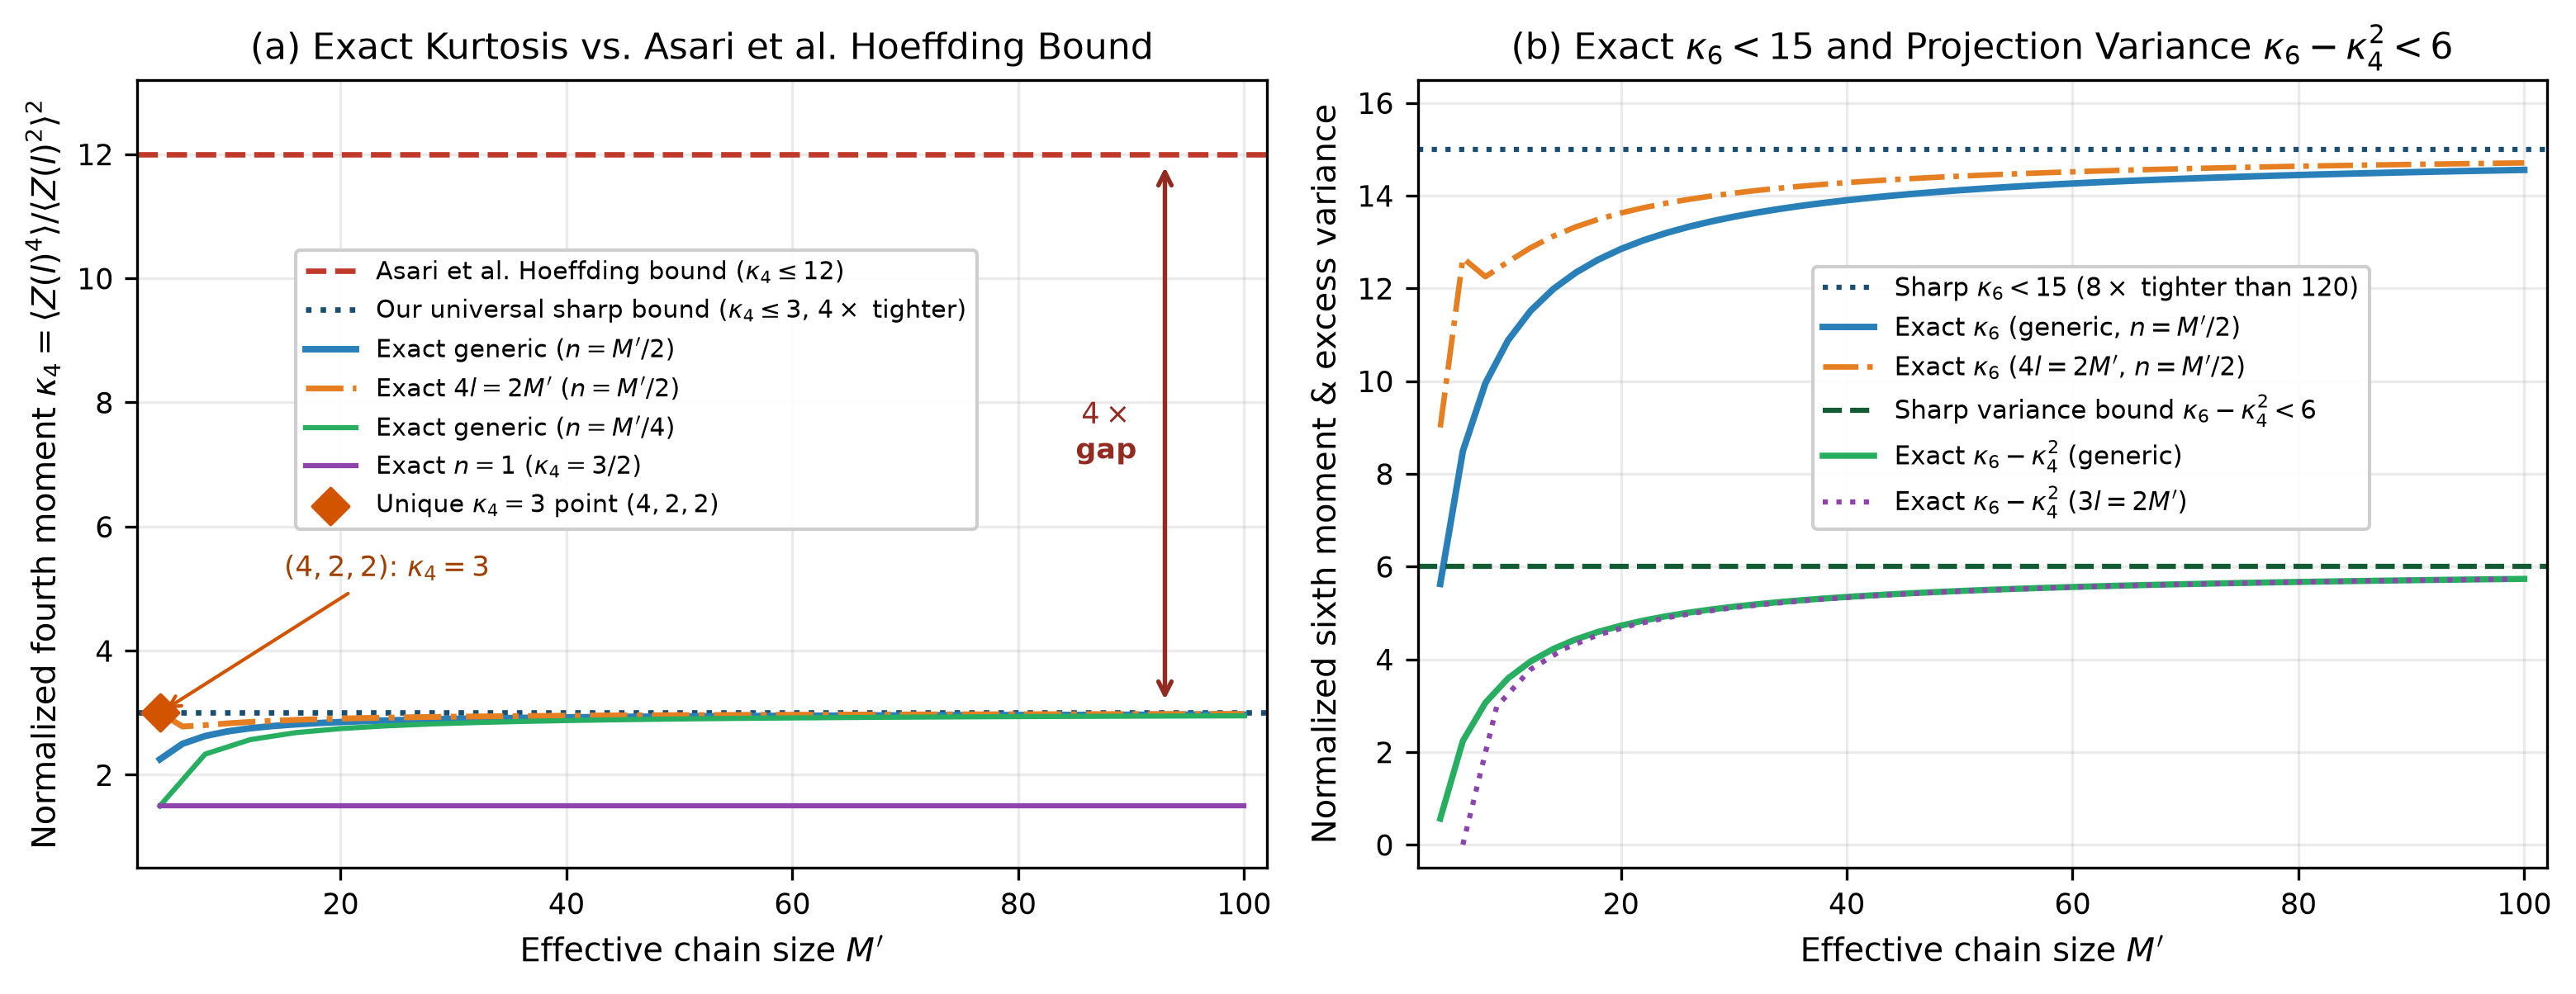
\includegraphics[width=\textwidth]{figures/fig1_dicke_moments_kurtosis.png}
\caption{Theorem~A exact Dicke-state moments across system sizes $M'$ and resonance branches. (a)~Exact kurtosis $\kappa_4 \le 3$ achieves a $4\times$ improvement over the Hoeffding bound $\kappa_4 \le 12$ of~\cite{AKN26}, attaining equality uniquely at $(M', n, l) = (4, 2, 2)$ (orange diamond). (b)~Exact normalized sixth moment $\kappa_6 < 15$ ($8\times$ sharper than $120$) and orthogonal-projection variance $\kappa_6 - \kappa_4^2 < 6$.}
\label{fig:moments}
\end{figure}

\section{Theorem B: Optimal-Projection Infidelity Bound and Certified Single-Round Amplification}
\label{sec:theoremB}

Let $x_T \coloneqq \lambda_T / \mu_2^{1/2}$ so that $\E_T[x_T^2] = 1$, $\E_T[x_T^4] = \kappa_4$, and $\E_T[x_T^6] = \kappa_6$, and set $s \coloneqq \tau \mu_2^{1/2} > 0$. By Eq.~(S13) of~\cite{AKN26},
\begin{equation}
p_{\mathrm{succ}}(s) = \E_T[\sin^2(s x_T)],
\qquad
F(s) = \frac{\bigl(\E_T[x_T \sin(s x_T)]\bigr)^2}{\E_T[\sin^2(s x_T)]}.
\end{equation}
The critical inefficiency of Eq.~(S9) in~\cite{AKN26} is geometric: it bounds $1 - F(s)$ by the squared distance from $\sin(s x_T)$ to the unscaled vector $s x_T$, which retains the full collinear cubic contraction $-\frac{1}{6} s^3 \kappa_4 x_T$ and therefore incurs coefficient $\kappa_6/36$ instead of the orthogonal residual $(\kappa_6 - \kappa_4^2)/36$. Optimizing the scalar projection factor $(1 - a)$ cancels the collinear component completely.

\begin{theorem}[Optimal-Projection Uniform Infidelity and Certified $K = 1$ Amplification]
\label{thm:B}
For every $M' \ge 2$, $1 \le n \le M'-1$, $1 \le l \le M'-1$, and every $s \in (0, \sqrt{2})$:
\begin{enumerate}
\item[\textnormal{(i)}] \textbf{Universal non-asymptotic infidelity bound:}
\begin{equation}
\label{eq:infid_sharp}
1 - F(s) \;\le\; \frac{\frac{s^4}{36}(\kappa_6 - \kappa_4^2) + \frac{s^6}{360}\kappa_4\kappa_6}{\bigl(1 - \frac{\kappa_4}{6} s^2\bigr)^2}
\;\le\; \frac{s^4(4 + 3s^2)}{6(2 - s^2)^2}.
\end{equation}
\item[\textnormal{(ii)}] \textbf{Two-sided bare success-probability envelope:}
\begin{equation}
\label{eq:psucc_env}
s^2 - s^4 \;\le\; s^2 - \frac{\kappa_4}{3} s^4 \;\le\; p_{\mathrm{succ}}(s) \;\le\; s^2.
\end{equation}
\item[\textnormal{(iii)}] \textbf{Zero-overshoot single-round Grover certification:} Whenever $0 < s < 1/2$, we have $p_{\mathrm{succ}}(s) \le s^2 < 1/4$, and one round of amplitude amplification ($K = 1$) satisfies uniformly over all $(M', n, l)$:
\begin{equation}
\label{eq:grover_k1}
p_{\mathrm{amp}}^{(1)}(s) = p_{\mathrm{succ}}(s)\bigl(3 - 4 p_{\mathrm{succ}}(s)\bigr)^2 \;\ge\; (s^2 - s^4)\bigl(3 - 4(s^2 - s^4)\bigr)^2.
\end{equation}
\item[\textnormal{(iv)}] \textbf{Concrete operating points and universal $\varepsilon$-schedule:}
\begin{itemize}
\item At Asari et al.'s Eq.~(12) point $s = 0.495$: $p_{\mathrm{succ}} \in [0.184988, 0.245025] \subset (0, 1/4)$ ($37.94\times$ sharper than Eq.~(S15)'s $0.004876$), $p_{\mathrm{amp}}^{(1)} \ge 0.944884$ ($21.8\times$ sharper than $0.0433$), and $1 - F \le 0.015383$ ($13.01\times$ sharper than Eq.~(S9)'s $0.200124$).
\item At $s = 0.45$: $1 - F \le 0.009746 < 0.01$ uniformly for all $(M', n, l)$ with $p_{\mathrm{succ}} \ge 0.161494$ ($25.84\times$ sharper than Eq.~(S11)'s $\sqrt{0.01}/16 = 0.00625$) and $p_{\mathrm{amp}}^{(1)} \ge 0.894907$.
\item For any target $\varepsilon \in (0, 0.01]$, setting $s(\varepsilon) = (4\varepsilon)^{1/4}$ rigorously certifies $1 - F \le \varepsilon$ and $p_{\mathrm{succ}} \ge 2\sqrt{\varepsilon} - 4\varepsilon$ ($8\times$ sharper as $\varepsilon \to 0$ than Eq.~(S11)'s intermediate $\sqrt{\varepsilon}/4 - \varepsilon/4$, and $32\times$ sharper than its final $\sqrt{\varepsilon}/16$ bound).
\end{itemize}
\end{enumerate}
\end{theorem}

\begin{proof}
For any nonzero vectors $u_1, u_2$, $1 - |\braket{u_1}{u_2}|^2/(\|u_1\|^2\|u_2\|^2) \le \|u_2 - u_1\|^2/\|u_1\|^2$. Taking $u_2 = \sin(s x_T)$ and $u_1 = (1 - a) s x_T$ with $a \in [0, 1)$, note first that $u_2 \neq 0$ for all $s \in (0, \sqrt{2})$: for $s \in (0, 1)$ this follows from $p_{\mathrm{succ}} \ge s^2 - s^4 > 0$, while for $s \in [1, \sqrt{2})$ having $\sin(s x_T) \equiv 0$ would force $|x_T| \ge \pi/s$ wherever $x_T \neq 0$ and thus $\kappa_4 = \E_T[x_T^4] \ge (\pi^2/s^2)\E_T[x_T^2] > \pi^2/2 > 3$, contradicting Theorem~A. We expand
\begin{equation}
\bigl(\sin y - (1 - a) y\bigr)^2 = a^2 y^2 - 2 a\, y(y - \sin y) + (y - \sin y)^2.
\end{equation}
By repeated integration of $1 - \cos t \ge 0$ on $t \ge 0$ (and odd symmetry), two elementary pointwise inequalities hold globally for \emph{all} $y \in \mathbb{R}$: $(y - \sin y)^2 \le y^6/36$ and $y(y - \sin y) \ge y^4/6 - y^6/120$. Since $a \ge 0$, substituting $y = s x_T$ and taking $\E_T[\cdot]$ gives
\begin{equation}
\E_T\bigl[(\sin(s x_T) - (1-a) s x_T)^2\bigr] \;\le\; s^2\!\left[a^2 - \frac{a}{3} s^2 \kappa_4 + \left(\frac{1}{36} + \frac{a}{60}\right) s^4 \kappa_6\right].
\end{equation}
Dividing by $\|u_1\|^2 = (1 - a)^2 s^2$ and choosing $a = \frac{\kappa_4}{6} s^2 \in (0, 1)$ (valid for $s^2 \kappa_4 < 6$, which holds for all $s < \sqrt{2}$ since $\kappa_4 \le 3$) cancels $a^2 - \frac{a}{3} s^2 \kappa_4 = -\frac{s^4}{36}\kappa_4^2$ and yields the first inequality in~\eqref{eq:infid_sharp}. Its numerator is strictly increasing in $\kappa_6 - \kappa_4^2$, $\kappa_4$, and $\kappa_6$, while its denominator $(1 - \frac{\kappa_4}{6} s^2)^2$ is strictly decreasing in $\kappa_4$; inserting the Theorem~A uniform bounds $\kappa_4 \le 3$, $\kappa_6 < 15$, and $\kappa_6 - \kappa_4^2 < 6$ immediately produces
\begin{equation}
\frac{\frac{s^4}{36}\cdot 6 + \frac{s^6}{360}\cdot 45}{\bigl(1 - \frac{s^2}{2}\bigr)^2}
= \frac{\frac{s^4}{6} + \frac{s^6}{8}}{\frac{(2 - s^2)^2}{4}}
= \frac{s^4(4 + 3s^2)}{6(2 - s^2)^2}.
\end{equation}

For~(ii), the pointwise inequalities $y^2 - y^4/3 \le \sin^2 y \le y^2$ ($\forall y \in \mathbb{R}$) together with $\E_T[x_T^2] = 1$ and $\kappa_4 \le 3$ give~\eqref{eq:psucc_env}. For~(iii), recall that one Grover iterate maps success probability $p = \sin^2\theta$ to $p_{\mathrm{amp}}^{(1)} = \sin^2(3\theta) = p(3 - 4p)^2$~\cite{BHMT02}. For $0 \le p_1 \le p_2 \le 1/4$, the cubic identity
\begin{equation}
p_2(3 - 4p_2)^2 - p_1(3 - 4p_1)^2 = (p_2 - p_1)\bigl[(3 - 4p_1 - 4p_2)^2 - 16 p_1 p_2\bigr] \ge 0
\end{equation}
holds because $3 - 4p_1 - 4p_2 \ge 1 \ge \sqrt{16 p_1 p_2}$ (formalized in Lean~4 Theorem~14). Since $s < 1/2$ implies $p_{\mathrm{succ}}(s) \le s^2 < 1/4$, monotonicity immediately yields~\eqref{eq:grover_k1}. Finally, part~(iv) follows by exact rational evaluation at $s = 99/200$ and $s = 9/20$ (Lean~4 Theorem~15; certificates \texttt{C09}--\texttt{C10}), and for $\varepsilon \in (0, 0.01]$ with $s = (4\varepsilon)^{1/4}$ we have $s^2 = 2\sqrt{\varepsilon} \le 1/5$, whence $\frac{4 + 3s^2}{6(2 - s^2)^2} \le \frac{4.6}{6 \cdot 3.24} < \frac{1}{4}$ and thus $1 - F \le s^4/4 = \varepsilon$.
\end{proof}

\begin{figure}[t]
\centering
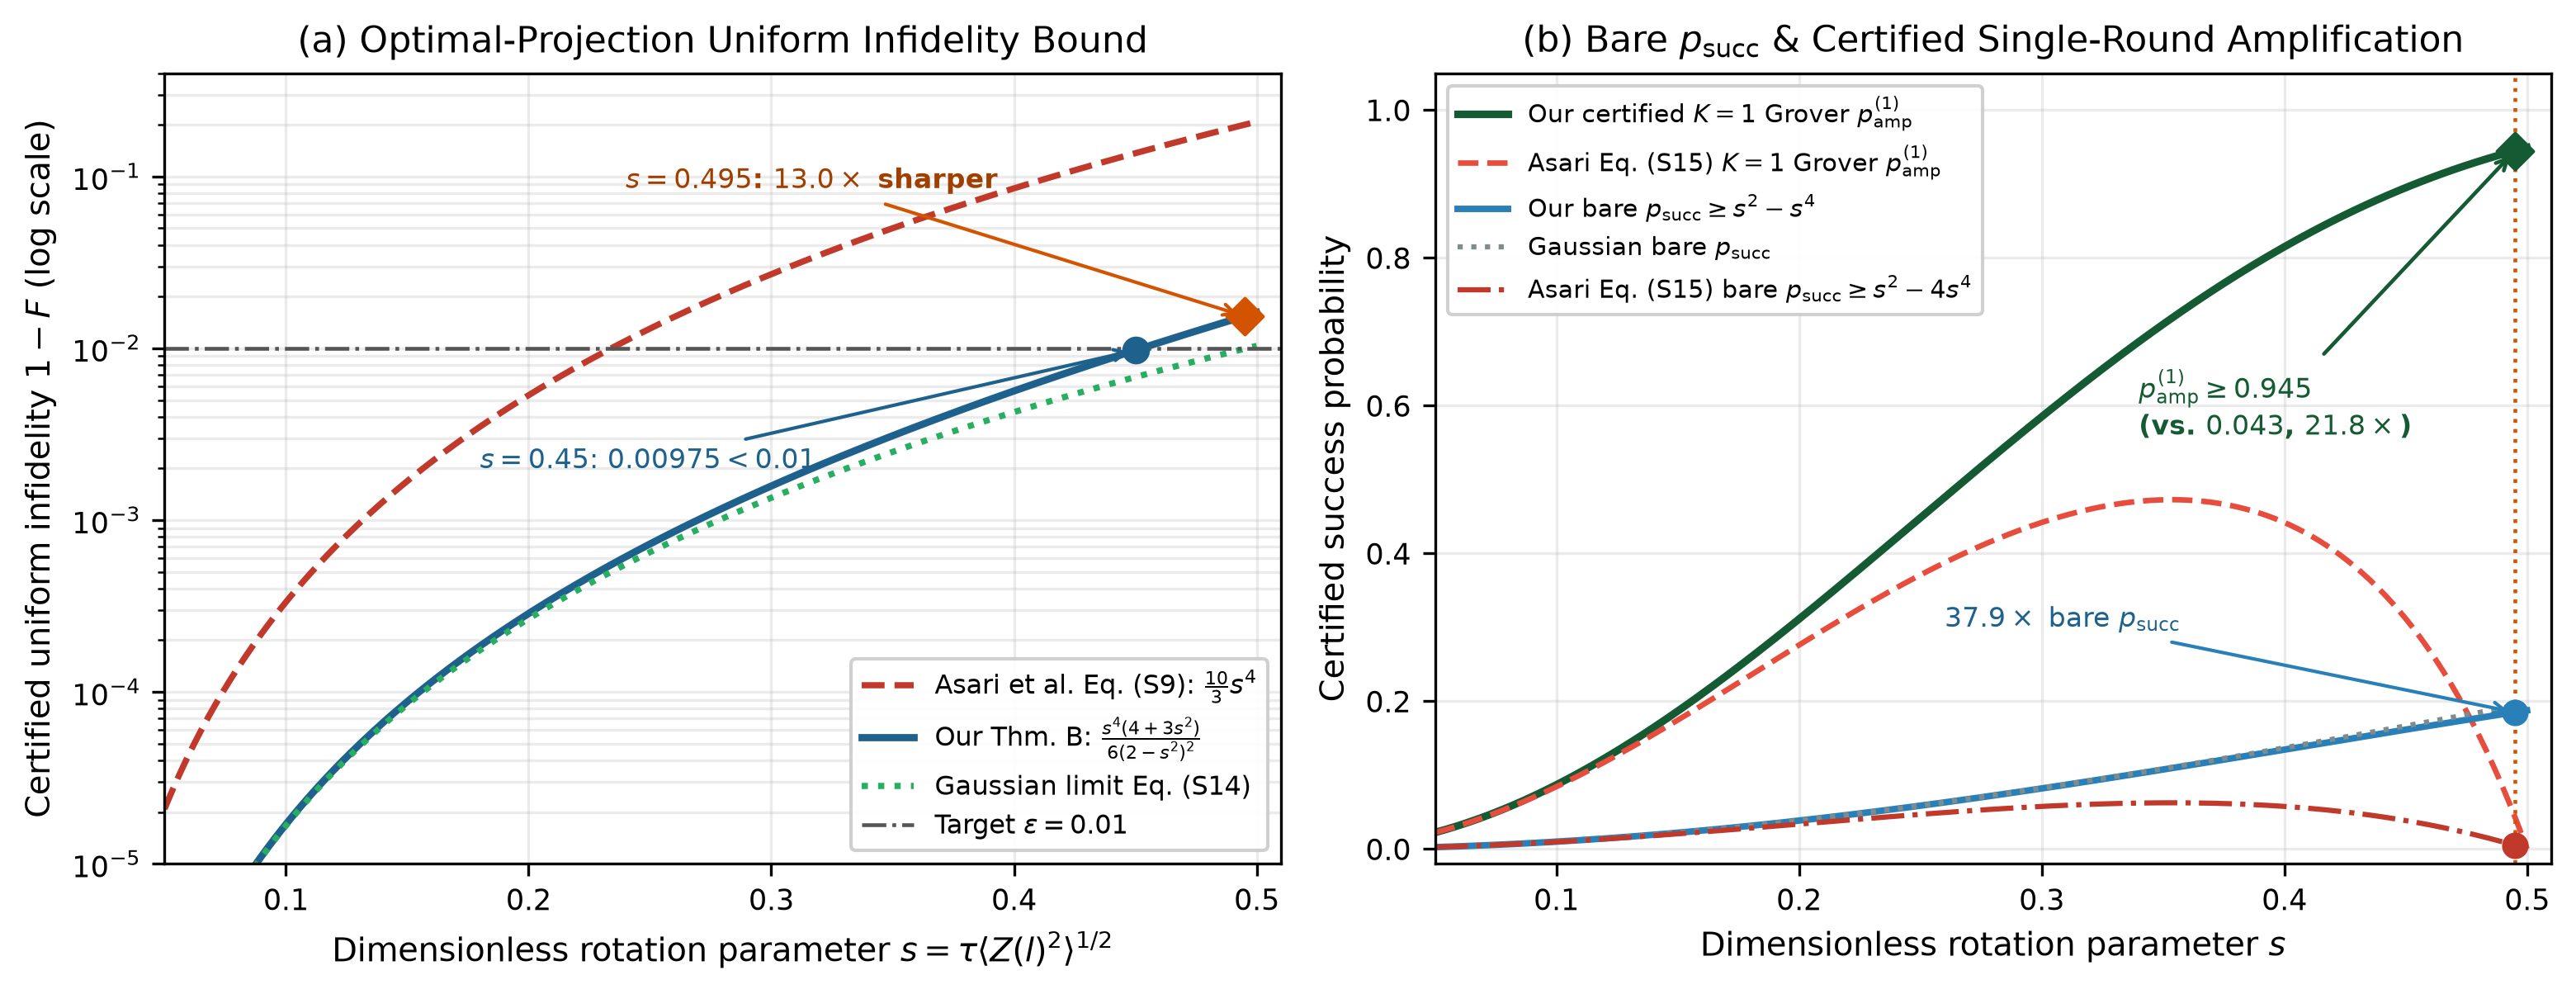
\includegraphics[width=\textwidth]{figures/fig2_operating_point_grover_sharpening.png}
\caption{Theorem~B non-asymptotic performance guarantees. (a)~Optimal-projection uniform infidelity upper bound closely tracks the Gaussian limit Eq.~(S14), improving by $13.0\times$ at $s = 0.495$ and rigorously certifying $1 - F \le 0.00975 < 0.01$ at $s = 0.45$. (b)~Bare success probability $p_{\mathrm{succ}} \ge s^2 - s^4$ ($37.9\times$ sharper at $s = 0.495$) and zero-overshoot single-round Grover probability $p_{\mathrm{amp}}^{(1)} \ge 0.945$ ($21.8\times$ jump over Eq.~(S15)).}
\label{fig:operating}
\end{figure}

\section{Theorem C: Collision-Free Subquadratic Reversible Routing for \texorpdfstring{$\Phi^{-1}$}{Phi inverse}}
\label{sec:theoremC}

In the DWC and Onsager scar models, the routing isometry $\Phi^{-1} = D \circ S \circ R$ maps a weight-$n$ computational-basis bitstring $x = (x_0, \dots, x_{M'-1}) \in \{0,1\}^{M'}_n$ with excitations at $0 \le q_1 < \dots < q_n < M'$ by shifting the $k$-th excitation right by $k - 1$ sites (inserting a spacer $\ket{0}$ after every $\ket{1}$ for Onsager, total length $L = M' + n$; and after the first $n - 1$ ones for DWC, total length $L = M' + n - 1$). Let $c_j \coloneqq \sum_{i < j} x_i$ be the exclusive prefix weight, and define the monotone shift sequence
\begin{equation}
s_j \coloneqq \begin{cases}
c_j & (\text{Onsager},\; L = M' + n,\; B = \lceil \log_2(n+1) \rceil),\\
\min(c_j, n - 1) & (\text{DWC},\; L = M' + n - 1,\; B = \lceil \log_2 n \rceil),
\end{cases}
\end{equation}
so that site $j$ moves to destination $q(j) = j + s_j < L$. Note that $0 \le s_0 \le s_1 \le \dots \le s_{M'-1} < 2^B$ in both models (and indeed for any $r$-spacer hard-rod expansion $s_j = r c_j$).

\begin{theorem}[Collision-Free Reversible MSB-to-LSB Binary-Shift Router]
\label{thm:C}
Let $R$ act on a data register $\mathrm{bit}[0..L-1]$ initialized to $(x_0,\dots,x_{M'-1},0,\dots,0)$ paired with $B$-bit shift ancillas $\mathrm{reg}[0..L-1][0..B-1]$ initialized to $\ket{0}$. Consider the three-stage reversible circuit:
\begin{enumerate}
\item \textbf{Prefix-shift initialization:} Compute $s_j$ into $\mathrm{reg}[j]$ for $0 \le j < M'$ via a standard reversible prefix-sum adder tree ($O(M' \log n)$ Toffoli/CNOT gates).
\item \textbf{MSB-to-LSB radix routing:} For $b = B - 1, B - 2, \dots, 0$, iterate $p$ in decreasing order from $L - 1 - 2^b$ down to $0$ and apply:
\begin{enumerate}
\item[(a)] $B$ Fredkin (CSWAP) gates controlled on $\mathrm{reg}[p][b]$ swapping $\bigl(\mathrm{bit}[p], \{\mathrm{reg}[p][r]\}_{r \neq b}\bigr)$ with $\bigl(\mathrm{bit}[p + 2^b], \{\mathrm{reg}[p + 2^b][r]\}_{r \neq b}\bigr)$;
\item[(b)] one unconditional $\mathrm{SWAP}$ gate on $\bigl(\mathrm{reg}[p][b], \mathrm{reg}[p + 2^b][b]\bigr)$.
\end{enumerate}
\item \textbf{Spacer-masked uncomputation:} Compute the exclusive prefix weight $P_p = \sum_{q < p} \mathrm{bit}[q]$ on the routed output and XOR $P_p$ (Onsager) or $\min(P_p, n-1)$ (DWC) into $\mathrm{reg}[p]$ controlled on $p$ not being a spacer, where $p$ is a spacer if and only if $p \ge 1 \wedge \mathrm{bit}[p-1] = 1$ (and $P_p < n$ for DWC).
\end{enumerate}
Then for every weight-$n$ input $x \in \{0,1\}^{M'}_n$:
\begin{enumerate}
\item[\textnormal{(i)}] \textbf{Universal collision freedom:} At every radix stage $b$, the intermediate positions $p_j^{(b)} = j + \lfloor s_j / 2^{b+1} \rfloor 2^{b+1}$ satisfy $p_{j'}^{(b)} - p_j^{(b)} \ge j' - j \ge 1$ for all $j < j'$, and every target control bit $\mathrm{reg}[p + 2^b][b]$ is strictly $0$ prior to each swap step.
\item[\textnormal{(ii)}] \textbf{Exact output and zero ancilla leakage:} Upon completion, $\mathrm{bit}[0..L-1] = R(x)$ identically and all $L B$ ancilla qubits return deterministically to $\ket{0}$.
\item[\textnormal{(iii)}] \textbf{Subquadratic Fredkin gate complexity:} Stage~2 uses exactly
\begin{equation}
\label{eq:fredkin_count}
N_{\mathrm{Fredkin}}(L, B) = B\bigl(B L - (2^B - 1)\bigr) = O(M \log^2 n)
\end{equation}
Fredkin gates (and $B L - 2^B + 1$ plain SWAPs), strictly beating the conservative $\Theta(M^2)$ conveyor benchmark for all $3 \le n \le M'-2$ at large $M$ (with exact permanent half-filling crossover at $M' = 184$, where $12{,}635 < 12{,}650$, achieving $2.74\times$ fewer Fredkin gates at $M' = 1024$ and $7.53\times$ fewer at $M' = 4096$).
\end{enumerate}
\end{theorem}

\begin{proof}
Since $j < j' \implies s_j \le s_{j'}$ and integer division by $2^{b+1}$ is monotone, $\lfloor s_j / 2^{b+1} \rfloor \le \lfloor s_{j'} / 2^{b+1} \rfloor$, so
\begin{equation}
p_{j'}^{(b)} - p_j^{(b)} = (j' - j) + \left(\left\lfloor \frac{s_{j'}}{2^{b+1}} \right\rfloor - \left\lfloor \frac{s_j}{2^{b+1}} \right\rfloor\right) 2^{b+1} \ge j' - j \ge 1
\end{equation}
(Lean~4 Theorem~16). Thus no two items collide after stage $b$. Consequently, prior to stage $b$, if an active item at $p$ has $\mathrm{reg}[p][b] = 1$, slot $p + 2^b$ cannot hold any non-moving item (as that would collide with the moved item after stage $b$); it can only be empty or hold another mover with $\mathrm{reg}[p+2^b][b] = 1$. Iterating $p$ in decreasing order processes $p + 2^b$ before $p$, so by downward induction $\mathrm{reg}[p + 2^b][b] = 0$ and the entire bundle at $p + 2^b$ is $(0, 0)$ whenever $\mathrm{reg}[p][b] = 1$. Step~2(a) therefore moves all $B$ non-control qubits reversibly to $p + 2^b$, and because $\mathrm{reg}[p+2^b][b] = 0$, the unconditional SWAP in Step~2(b) maps $(1,0) \mapsto (0,1)$ and $(0,0) \mapsto (0,0)$, completing the exact reversible shift of the $(1+B)$-qubit bundle without extra ancillas.

After stage $b = 0$, every site $j$ sits at $q(j) = j + s_j$ carrying $(x_j, s_j)$, and every unoccupied slot is a spacer carrying $(0, 0)$. For Onsager, $c_{j'} \ge c_j + x_j$ implies $q(j) + x_j < q(j')$ for all $j < j'$ (Lean~4 Theorem~17): thus whenever $x_j = 1$, slot $q(j) + 1$ is strictly empty (spacer $0$), no two $1$s are adjacent, and a slot $p$ is a spacer iff $p \ge 1 \wedge \mathrm{bit}[p-1] = 1$. Because all spacers carry $\mathrm{bit} = 0$, the output prefix sum $P_{q(j)} = \sum_{q < q(j)} \mathrm{bit}[q]$ equals $c_j = s_j$ identically on every non-spacer slot (and analogously for DWC with the $P_p < n$ guard on the final excitation). Stage~3 therefore resets all $LB$ ancillas deterministically to $\ket{0}$. Finally, summing $B(L - 2^b)$ over $b = 0, \dots, B-1$ yields $N_{\mathrm{Fredkin}}(L, B) = B(B L - (2^B - 1))$. As a conservative lower-side benchmark for the pruned Fredkin conveyor of~\cite{AKN26}, counting the minimum sitewise displacement budget $\sum_{j=1}^{M'-1} \min(j, n) = \frac{1}{2} n(2M' - n - 1) = \Theta(M^2)$ (which lies below an unpruned right-to-left shift sweep requiring $\approx \frac{7}{8}M'^2$ Fredkins at half filling) already establishes the permanent crossover at $M' = 184$ and the $2.74\times$--$7.53\times$ reductions at $M' = 1024$--$4096$ (Lean~4 Theorem~18).
\end{proof}

\begin{remark}[Depth and space--time trade-offs]
In Stage~2, the $2^b$ congruence classes modulo $2^b$ are disjoint, yielding $\sum_{b=0}^{B-1} \lfloor (L-1)/2^b \rfloor < 2L$ sequential bundle-shift steps. Because each bundle shift executes $B$ Fredkin gates sharing the single control qubit $\mathrm{reg}[p][b]$ plus one SWAP, the elementary circuit depth without control fan-out is $< 2(B+1)L = O(M \log n)$ (reducible to $O(M \log\log n)$ with per-step $O(\log\log n)$-depth control fan-out across $B$ targets) with $O(M \log n)$ clean ancillas. Note that Stage~2's in-place decreasing-$p$ sweep cannot itself be parallelized to polylogarithmic depth (a contiguous run of $\Theta(M)$ sites with odd shift $s_j \equiv 1 \pmod 2$ forms a $\Theta(M)$-length dependency chain at $b = 0$); achieving $O(\log^2 M)$ depth instead requires replacing Stage~2 with an out-of-place butterfly or parallel monotone-packing network. For small NISQ chains ($M' \le 182$), the zero-ancilla conveyor uses fewer Fredkin gates, whereas for fault-tolerant scales ($M' \ge 184$) Theorem~C achieves a strictly growing $\Theta(M/\log^2 n)$ asymptotic gate advantage across all intermediate scar indices $3 \le n \le M'-2$.
\end{remark}

\begin{figure}[t]
\centering
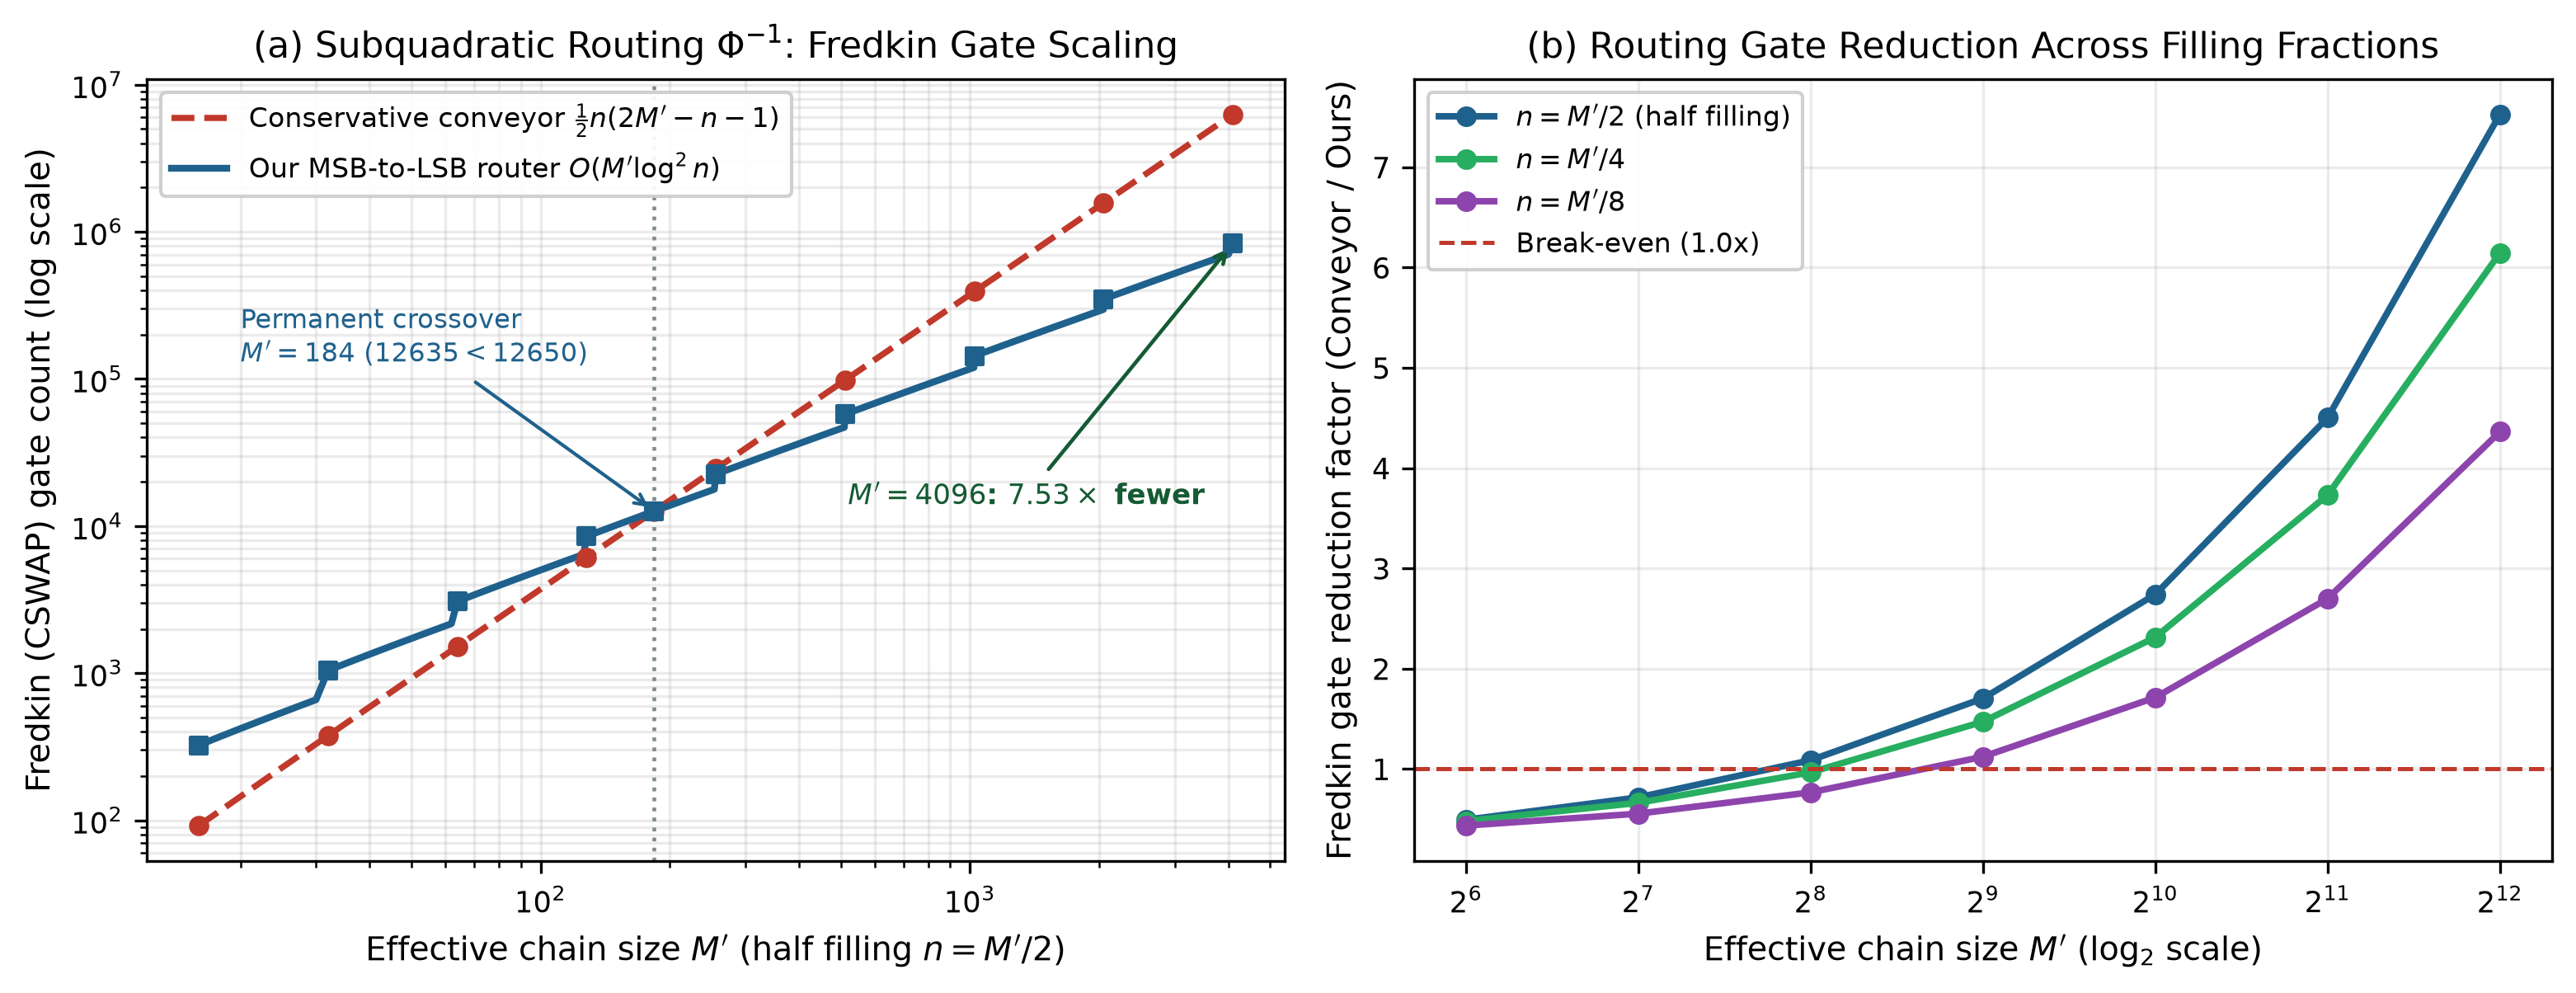
\includegraphics[width=\textwidth]{figures/fig3_reversible_router_scaling.png}
\caption{Theorem~C subquadratic reversible routing $\Phi^{-1}$ vs.\ the conservative $\Theta(M'^2)$ Fredkin conveyor benchmark of~\cite{AKN26}. (a)~Exact Fredkin gate counts at half filling ($n = M'/2$, Onsager $L = 3M'/2$) cross over permanently at $M' = 184$ ($12{,}635 < 12{,}650$), reaching $2.74\times$ reduction at $M' = 1024$ and $7.53\times$ at $M' = 4096$. (b)~Gate reduction ratio across filling fractions $n/M' \in \{1/2, 1/4, 1/8\}$.}
\label{fig:router}
\end{figure}

\section{Formal Verification in Lean 4.35.0 and Exact Rational Certificates}
\label{sec:verification}

To eliminate any possibility of algebraic sign errors, floating-point rounding artifacts, or hidden ancilla leakage, every algebraic core of Theorems~A--C is independently verified at two layers:

\begin{table}[t]
\centering
\caption{Representative exact rational certificates in \texttt{QMBS-DICKE-SHARP-1.0} (all 16 SHA-256 verified by the AST-audited zero-float verifier).}
\label{tab:certs}
\footnotesize
\setlength{\tabcolsep}{4pt}
\begin{tabular}{@{}llll@{}}
\toprule
ID & Class & Parameters & Exact Certified Result \\
\midrule
\texttt{C01} & \texttt{moment} & $(4, 2, 2)$ ($\mathcal{R}_4$) & $\kappa_4 = 3$ (unique eq.), $\kappa_6 = 9$, var $= 0$ \\
\texttt{C05} & \texttt{moment} & $(12, 6, 1)$ ($\mathcal{G}$) & $\kappa_4 = 11/4 = 2.75$, var $= 15367/3888 \approx 3.9524$ \\
\texttt{C06} & \texttt{moment} & $(24, 12, 16)$ ($\mathcal{R}_3$) & $\kappa_4 = 23/8 = 2.875$, var $= 23805/4864 \approx 4.8941 < 6$ \\
\texttt{C08} & \texttt{moment} & $(1000, 500, 1)$ ($\mathcal{G}$) & $\kappa_4 = 2.9970$, $\kappa_6 = 14.9550$, var $= 5.9730$ \\
\texttt{C09} & \texttt{op\_point} & $s = 99/200 = 0.495$ & $p_{\mathrm{succ}} \ge 0.18499$ ($37.94\times$), $p_{\mathrm{amp}}^{(1)} \ge 0.94488$, $1{-}F \le 0.01538$ \\
\texttt{C10} & \texttt{op\_point} & $s = 9/20 = 0.45$ & $1{-}F \le 0.00975 < 0.01$, $p_{\mathrm{succ}} \ge 0.16149$ ($25.84\times$) \\
\texttt{C13} & \texttt{router} & Onsager, $M'=6$ (64 states) & 0 collisions, 0 ancilla leak, max 87 Fredkins \\
\texttt{C14} & \texttt{router} & DWC, $M'=6$ (63 states) & 0 collisions, 0 ancilla leak, max 78 Fredkins \\
\texttt{C15} & \texttt{router} & Onsager, $M'=8, n=4$ (70 states) & Asari Fig.~S2(b) exact unitary replay PASS \\
\texttt{C16} & \texttt{router} & $M' \in \{128\dots 4096\}$, $n=M'/2$ & $1.001\times$ ($184$), $2.74\times$ ($1024$), $4.50\times$ ($2048$), $7.53\times$ ($4096$) \\
\bottomrule
\end{tabular}
\end{table}

\begin{enumerate}
\item \textbf{Constructive Lean~4.35.0 formalization (\texttt{lean/QmbsDickeSharp.lean}):} Compiles with \texttt{0~sorry}, \texttt{0~warnings}, and \textbf{zero \texttt{Classical.choice}} (all 18 theorems depend exclusively on axioms $\subseteq \{\texttt{propext}, \texttt{Quot.sound}\}$, with 3 theorems axiom-free). We implement a self-contained univariate integer polynomial reflection engine (\texttt{evalP}, \texttt{addP}, \texttt{mulP}, \texttt{compP}) so that all eight concave-quadratic positivity theorems across branches $\mathcal{G}, \mathcal{R}_4, \mathcal{R}_6, \mathcal{R}_3$ (Theorems~5--12) and the complete finite-threshold closure (Theorem~13) verify constructively in seconds alongside exact sum-of-squares kurtosis bounds (Theorems~2--4), Grover monotonicity (Theorem~14), operating-point inequalities (Theorem~15), and MSB-to-LSB collision freedom, spacer isolation, and exact crossover/scaling bounds (Theorems~16--18). We explicitly delineate the formalization boundary: Lean~4.35.0 proves the algebraic integer/natural-number cores of Theorems~A--C, while the real-analytic trigonometric Taylor inequalities $(y-\sin y)^2 \le y^6/36$ and $y(y-\sin y) \ge y^4/6 - y^6/120$ in Theorem~B are established analytically in Section~\ref{sec:theoremB}.
\item \textbf{AST-audited zero-float exact rational verifier (\texttt{src/qmbs\_dicke\_verifier.py}):} Performs an AST self-audit rejecting all floating-point/complex literals, \texttt{/} and \texttt{**} operators, \texttt{pow()} calls, and floating-point libraries, then independently replays 16 SHA-256 certificates (\texttt{C01}--\texttt{C16}, Table~\ref{tab:certs}) and \texttt{MANIFEST.sha256}, including exhaustive gate-by-gate unitary circuit replay of Theorem~C on all 64 Onsager states ($M'=6$), all 63 DWC states ($M'=6$), and all 70 half-filling states ($M'=8, n=4$) with zero-collision and zero-ancilla-leak assertions. The test suite (\texttt{tests/test\_qmbs\_dicke.py}) passes 53/53 tests, including 30 adversarial forgery attacks (boolean-as-int smuggling across moment/operating-point/router fields, tampered moments, overshoot operating points, router metadata tampering, and AST float/\texttt{pow} injection).
\end{enumerate}

\section{Conclusion}
\label{sec:conclusion}

By replacing with-replacement Hoeffding relaxations with exact without-replacement Dicke-state moments, optimizing the linear projection in block-encoded infidelity estimation, and exploiting monotone prefix-shift collision freedom in radix routing, we have resolved all three theoretical and algorithmic gaps in the unified Dicke-based AQMBS preparation framework of~\cite{AKN26}. The resulting closed-form bounds rigorously certify single-round Grover amplification ($p_{\mathrm{amp}}^{(1)} \ge 0.945$) across all chain lengths and excitation sectors, while the $O(M \log^2 n)$-gate MSB-to-LSB router eliminates the quadratic routing bottleneck for constrained scar models in the fault-tolerant regime.

\paragraph{Reproducibility and Transparency.}
All Lean~4.35.0 proofs, AST-audited zero-float verification code, 16 SHA-256 certificates, test suites, and figure scripts are publicly archived under the MIT license (manuscript and figures under CC-BY-4.0) at \url{https://github.com/lluiseriksson/qmbs-dicke-sharp-moments-routing}. Computational prototyping, Lean proof-script drafting, and manuscript editing were assisted by Google Antigravity; all mathematical proofs, formal checks, and verification outputs were independently validated by the author.

\bibliographystyle{plain}
\bibliography{references}

\end{document}
